\documentclass[11pt]{article}

\usepackage[margin=1in]{geometry}
\usepackage[T1]{fontenc}
\usepackage[utf8]{inputenc}
\usepackage{lmodern}
\usepackage{microtype}
\usepackage{amsmath,amssymb,amsthm}
\usepackage{mathtools}
\usepackage{array}
\usepackage{graphicx}
\graphicspath{{figures/}}
\usepackage{booktabs}
\usepackage{enumitem}
\usepackage[round]{natbib}
\usepackage[hidelinks]{hyperref}
\usepackage{cleveref}
\usepackage{placeins}

\newcommand{\HT}{\mathrm{HT}}
\newcommand{\HTp}{\mathrm{HT}^{+}}
\newcommand{\Otil}{\widetilde{O}}
\newcommand{\U}{\mathcal{U}}
\newcommand{\Prob}{\mathbb{P}}
\newcommand{\E}{\mathbb{E}}

\theoremstyle{plain}
\newtheorem{theorem}{Theorem}
\newtheorem{lemma}{Lemma}
\newtheorem{proposition}{Proposition}
\theoremstyle{definition}
\newtheorem{definition}{Definition}
\newtheorem{conjecture}{Conjecture}

\title{Quantum Walk Search for Marked Vertices as a Model of Cognitive Search:\\[0.3em]
\large From Semantic Memory Retrieval to Multi-Alternative Decision Making}
\author{[Student Name 1] \quad [Student ID 1]\\[0.2em]
[Student Name 2] \quad [Student ID 2]}
\date{EE5105 Special Topics in Quantum Information Science\\
Instructor: Prof. Shih-Han Hung \quad Fall 2026}

\begin{document}

\maketitle

\begin{abstract}
We use the Ambainis--Gily\'en--Jeffery--Kokainis (AGJK) marked-vertex search
algorithm as the technical core of a process-level model of cognitive search.
Numerically, the quantum search time scales as $T_q\sim \HT^{0.44\text{--}0.52}$
on complete graphs, cycles, grids, and hypercubes, and independent targets are
easier than clustered ones. A large extended-hitting-time gap appears only in
the AGJK adversarial torus construction, not for generic clustered targets. On
a toy semantic graph, continuous-time quantum walks produce larger and later
target activation than classical diffusion, especially for cross-community
targets. In a multi-alternative decision graph, coupling two options shifts the
quantum choice probability toward the uncoupled option (from $1/3$ to $0.50$
on a symmetric three-option graph), whereas the classical choice stays
uniform; this holds only
under phase-free readouts, and we show that a first-threshold readout is
dominated by the oscillation phase. A partial-
measurement sweep shows that the pure walk has the highest peak but needs it
to be timed; when a measurement can end the search, an intermediate rate
($p\approx0.2$--$0.3$) finds clustered targets by a moderate deadline with
higher probability than either the pure quantum or the classical walk
($0.45$ versus $0.33$ at $T=40$ on a grid).
The project connects quantum-walk complexity to testable model-level predictions
without claiming a biological quantum advantage.
\end{abstract}

\section{Introduction}
\label{sec:introduction}

Quantum cognition models judgment, memory, and decision making with the
mathematical structure of quantum probability. It does not claim that the brain
is a quantum computer. Instead, it uses Hilbert spaces, superposition, and
interference to capture contextuality, order effects, and evidence accumulation
that classical probability handles awkwardly \citep{pothos2022,busemeyer2024}.
Quantum walks are a natural process-level ingredient: a walker on a semantic or
decision graph represents unfolding evidence, a marked vertex represents a
target memory or an option, and the walk's statistics define response times and
choice probabilities \citep{chen2022,huang2022,pavone2025}.

The missing link is algorithmic structure. The quantum-walk literature on
search focuses on worst-case query and time complexity: given a graph and a
marked set, how quickly can one detect or find a marked vertex? The quantum
cognition literature focuses on explaining behavioral signatures. The two
bodies of work meet mostly through the metaphor that a quantum walk is an
evidence accumulator. The marked-vertex search problem itself---especially its
behavior with multiple marked vertices---is rarely used as a formal model of
cognitive search.

This project uses the Ambainis--Gily\'en--Jeffery--Kokainis (AGJK) algorithm as
the technical core \citep{agjk2019}. AGJK gives a quantum walk algorithm that
finds a marked vertex on an arbitrary graph, for an arbitrary marked set, with
a quadratic speedup over the classical hitting time up to logarithmic factors.
It also isolates the extended hitting time $\HT^+$, which can be much larger
than $\HT$ when there are multiple marked vertices. That structure maps
naturally onto cognitive search with several targets and onto multi-alternative
choice, where similar options compete and context changes the choice
distribution.

We ask three questions.
\begin{enumerate}[leftmargin=1.4em]
  \item \textbf{Mapping.} How do $\HT$, $\HT^+$, the spectral gap, and the
  success probability map onto response time, choice probability, and
  deliberation speed on a semantic or decision graph?
  \item \textbf{Structure.} How do the number and arrangement of marked
  vertices---single, independent, clustered---change the quantum versus
  classical search time and success probability? Can $\HT^+$ formalize
  multi-alternative decision difficulty and context effects?
  \item \textbf{Noise.} How does partial measurement or decoherence erode the
  quantum advantage, and is there an optimal ``introspection'' level that
  maximizes success probability or decision speed?
\end{enumerate}

\Cref{fig:architecture} summarizes the three layers of the project: the QIS
core, the graph model, and the cognitive quantities derived from the walk.

\begin{figure}[t]
  \centering
  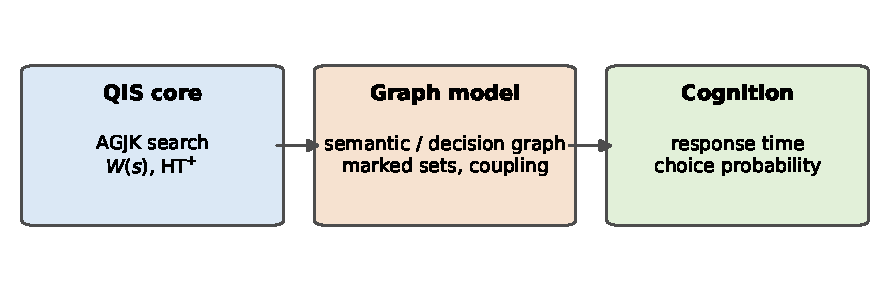
\includegraphics[width=0.92\linewidth]{figures/fig_architecture.pdf}
  \caption{Three-layer architecture. The AGJK search core supplies the walk
  operator and the hitting-time structure; the graph layer maps concepts or
  options to vertices and marked sets; the cognitive layer turns walk statistics
  into response times and choice probabilities.}
  \label{fig:architecture}
\end{figure}

The project makes four contributions. First, we implement the Szegedy walk,
the interpolated walk $W(s)$, and the AGJK extended hitting time, and we verify
the $\widetilde O(\sqrt{\HT})$ scaling numerically on complete graphs, cycles,
grids, and hypercubes. Second, we compare single, independent, and clustered
marked sets. We show that independent targets are easier, that clustered
targets give only a modest reduction of the hitting time relative to a single
target ($\approx3\%$ on the barbell, $\approx17\%$ on the $8\times8$ grid), and that the dramatic $\HT^+\gg\HT$ gap
requires the adversarial periodic arrangement of AGJK rather than clustering
alone. Third, we build a semantic graph and a multi-branch decision graph and
turn the walk statistics into target activation, response time, and choice
probability. Fourth, we add a partial-measurement model and show that
single-deadline comparisons are dominated by the phase of the quantum
oscillation. With deadline-free readouts, the pure walk keeps the highest timed
peak, while at moderate deadlines an intermediate measurement rate that can
stop the search finds clustered targets faster than both the pure quantum and
the classical walk.

The paper is organized as follows. \Cref{sec:background} reviews classical and
quantum walks and the quantum cognition literature. \Cref{sec:theory} collects
the formal definitions and the AGJK results we use. \Cref{sec:cognitive-model}
states the cognitive mapping and its assumptions. \Cref{sec:methods} describes
the graph families, protocols, and metrics. \Cref{sec:results} reports E1--E5.
\Cref{sec:discussion} discusses interpretation, limitations, and future work.

\section{Background}
\label{sec:background}

\subsection{Classical random walks and hitting times}
\label{sec:background-classical}

Let $G=(V,E)$ be a connected graph with $n=\lvert V\rvert$ vertices and let
$P$ be a row-stochastic transition matrix. A probability row vector $\pi$ is
stationary if $\pi P=\pi$. For a reversible chain, detailed balance holds:
$\pi_xP_{xy}=\pi_yP_{yx}$ for all $x,y$.

Given a non-empty marked set $M\subset V$, the hitting time is the expected
number of steps needed to reach $M$ from the stationary distribution,
\begin{equation}
  \HT(P,M)=\mathbb{E}_{X_0\sim\pi}\left[\min\{t\ge0:X_t\in M\}\right].
\end{equation}
For computations we use the equivalent conditioned form
\begin{equation}
  \HT(P,M)=\frac{1}{1-p_M}\sum_{x\notin M}\pi_x h_x,
  \qquad h_x=1+\sum_yP_{xy}h_y,\quad x\notin M,
  \label{eq:background-ht}
\end{equation}
with $p_M=\sum_{x\in M}\pi_x$. The linear system in \eqref{eq:background-ht}
is small for the graphs in this paper and can be solved directly. Standard
examples are $\HT=\Theta(N)$ on the complete graph, $\HT=\Theta(N^2)$ on the
cycle, and $\HT=\Theta(N\log N)$ on the two-dimensional grid; the hypercube has
$\HT=\Theta(N)$, and our data ($N=8$--$64$) give $\HT/N\approx1.15$--$1.34$.

\subsection{Szegedy walks and the detection--finding gap}
\label{sec:background-szegedy}

A Szegedy walk lifts a Markov chain to a unitary operator on two vertex
registers. With the convention used by AGJK,
\begin{equation}
  V(P)\lvert\bar0\rangle\lvert x\rangle
  =\sum_y\sqrt{P_{xy}}\lvert y,x\rangle,
  \qquad
  W(P)=V^\dagger(P)\,\mathrm{Shift}\,V(P)\,\mathrm{Ref},
  \label{eq:background-szegedy}
\end{equation}
where $\mathrm{Shift}\lvert x,y\rangle=\lvert y,x\rangle$ and
$\mathrm{Ref}=(2\lvert\bar0\rangle\langle\bar0\rvert-I)\otimes I$. The
discriminant matrix is
\begin{equation}
  D_{xy}=\sqrt{P_{xy}P_{yx}}
  =\langle\bar0|\langle x|W(P)|\bar0\rangle|y\rangle.
\end{equation}
For a reversible chain, $D=\mathrm{diag}(\pi)^{1/2}P\,\mathrm{diag}(\pi)^{-1/2}$,
so $D$ and $P$ share their spectrum and $D$ is symmetric.

Szegedy's search algorithm detects a marked vertex in
$O(\sqrt{\HT})$ steps. Detection is not the same as finding: measuring the
final state need not return a marked vertex. The gap is especially visible
when there are multiple marked vertices. This is the starting point of AGJK.

\subsection{The AGJK algorithm and extended hitting time}
\label{sec:background-agjk}

AGJK introduce the absorbing walk $P'$ and the interpolated walk
$P(s)=(1-s)P+sP'$, which stays at a marked vertex with probability $s$ instead
of moving. The corresponding quantum walk $W(s)$ uses an ancilla to record
whether the current vertex is marked. AGJK define the extended hitting time
$\HT^+$ through the eigenvalues and eigenvectors of the discriminant matrix
$D(s)$; if there is a single marked vertex, $\HT^+=\HT$, but with multiple
marked vertices $\HT^+$ can be much larger.

Two algorithms are given. The simpler one runs $W(s)$ for $O(\sqrt{\HT})$
steps and is supported by a numerical conjecture (Conjecture~3 in the paper):
for some $s$ and $t=O(\sqrt{\HT})$, measuring the vertex register returns a
marked vertex with constant probability. The proved algorithm combines the
interpolated walk with quantum fast-forwarding and achieves
$\widetilde O(\sqrt{\HT})$ time for any graph and any marked set
\citep{agjk2019}. We implement and test the first algorithm numerically; we
cite the second as the theoretical guarantee and do not re-prove it.

\subsection{Quantum cognition and quantum walks}
\label{sec:background-cognition}

Quantum cognition replaces classical probability with quantum probability in
models of judgment and decision. Pothos and Busemeyer review the program and
its explanations of order effects, conjunction and disjunction effects, and
contextuality \citep{pothos2022,busemeyer2024}. The models are usually
process-level: they do not assume that the brain implements a quantum circuit.

Quantum walks enter this literature in several ways. Chen, Ferro, and Sornette
use discrete-time quantum walks as evidence accumulators and discuss how
partial measurement produces decoherence \citep{chen2022}. Huang and Busemeyer
propose a quantum walk framework for multi-alternative decision making
\citep{huang2022}. Pavone and Faro use continuous-time quantum walks on
semantic graphs to model the emergence of insight through interference
\citep{pavone2025}. Epping et al.\ develop an open-system model of choice and
response time \citep{epping2023}, and Widdows et al.\ give quantum circuit
components for cognitive decision-making \citep{widdows2023}.

\begin{table}[t]
  \centering
  \small
  \begin{tabular}{@{}p{0.23\linewidth}p{0.25\linewidth}p{0.25\linewidth}p{0.19\linewidth}@{}}
    \toprule
    Paper & Model & Cognitive phenomenon & Role here \\
    \midrule
    AGJK 2019 & quantum walk search & marked-vertex search, $\HT^+$ & QIS core \\
    Chen et al.\ 2022 & DTQW & evidence accumulation, decoherence & measurement model \\
    Huang--Busemeyer 2022 & quantum walk & multi-alternative choice & decision mapping \\
    Pavone--Faro 2025 & CTQW on semantic graphs & insight, interference & semantic experiment \\
    Pothos--Busemeyer 2022 & quantum probability & context, order effects & motivation \\
    Epping et al.\ 2023 & open-system model & choice and response time & noise interpretation \\
    \bottomrule
  \end{tabular}
  \caption{Literature map. The technical core is AGJK; the other papers supply
  the cognitive interpretation and the measurement/noise models.}
  \label{tab:literature}
\end{table}

\subsection{The gap}
\label{sec:background-gap}

The two literatures meet at the level of metaphor but not at the level of
algorithmic structure. Quantum-walk search papers analyze worst-case
complexity and spectral quantities but do not ask what those quantities mean
for a cognitive process. Quantum-cognition papers use walks as evidence
accumulators but rarely exploit the marked-set structure, the extended hitting
time, or the difference between detection and finding. This paper treats the
marked-vertex search problem as a process model and uses its structural
quantities---$\HT$, $\HT^+$, the spectral gap, and the success curve---as the
bridge between the two literatures.

\section{Theory}
\label{sec:theory}

\subsection{Reversible chains and the discriminant matrix}
\label{sec:theory-discriminant}

Let $P$ be an ergodic reversible Markov chain with stationary distribution
$\pi$. The discriminant matrix is
\begin{equation}
  D_{xy}=\sqrt{P_{xy}P_{yx}},
  \qquad
  D=\mathrm{diag}(\pi)^{1/2}P\,\mathrm{diag}(\pi)^{-1/2}.
  \label{eq:discriminant}
\end{equation}
For reversible $P$, $D$ is symmetric and has the same spectrum as $P$; the
vector $\sqrt{\pi}$ is a left eigenvector with eigenvalue $1$. The Szegedy walk
\eqref{eq:background-szegedy} satisfies
\begin{equation}
  \langle\bar0|\langle x|W(P)|\bar0\rangle|y\rangle=D_{xy}.
\end{equation}
The following standard spectral fact is used repeatedly. If
$D=\sum_k\lambda_k|v_k\rangle\langle v_k|$, then the nontrivial eigenvalues of
$W(P)$ are $e^{\pm i\theta_k}$ with $\lambda_k=\cos\theta_k$, and the
corresponding eigenvectors lie in the span of
$\{\lvert\bar0\rangle\lvert x\rangle\}_{x\in V}$ and its image under $V(P)$.
This is the Szegedy spectral lemma; we use it as a statement and do not
reprove it.

\subsection{Classical and extended hitting times}
\label{sec:theory-ht}

For a marked set $M$ with stationary mass $p_M=\sum_{x\in M}\pi_x$, the
classical hitting time can be written in spectral form as
\begin{equation}
  \HT(P,M)=\frac{1}{1-p_M}\sum_{k=1}^{n-|M|}
  \frac{\lvert\langle v'_k\rvert\sqrt{\pi_U}\rangle\rvert^2}{1-\lambda'_k},
  \label{eq:ht-spectral}
\end{equation}
where $\lambda'_k$ are the non-unit eigenvalues of $D(1)$ and
$\sqrt{\pi_U}$ is the subnormalized vector with entries $\sqrt{\pi_x}$ for
$x\notin M$.

AGJK replace $D$ by the discriminant matrix $D(s)$ of the interpolated walk and
define
\begin{equation}
  \HT(s)=\frac{1}{1-p_M}\sum_{k=1}^{n-1}
  \frac{\lvert\langle v_k(s)\rvert\sqrt{\pi_U}\rangle\rvert^2}{1-\lambda_k(s)},
  \qquad
  \HTp=\lim_{s\to1}\HT(s),
  \label{eq:ht-plus-theory}
\end{equation}
where $D(s)=\sum_k\lambda_k(s)|v_k(s)\rangle\langle v_k(s)|$ and
$\lambda_n(s)=1$. For a single marked vertex, $\HTp=\HT$. For multiple marked
vertices, \eqref{eq:ht-plus-theory} can be much larger than \eqref{eq:ht-spectral}.

The canonical example is an $N\times N$ torus with marked set
\begin{equation}
  M=M_1\cup M_2,\qquad
  M_1=\{(j_1d_1,j_2d_1):0\le j_1,j_2<k_1\},\quad
  M_2=\{(j_1d,j_2d):0\le j_1,j_2<N/d\},
  \label{eq:adversarial-set}
\end{equation}
with $d_1\mid d\mid N$ and the scale separation of AGJK. The set $M_1$ is a
dense cluster and $M_2$ is a sparse periodic grid. For suitable parameters,
$\HT=\widetilde O(d^2)$ while $\HTp=\Omega(N^2)$; this is AGJK's asymptotic
statement. Our numerics ($L=18$--$36$) can show growth of $\HTp/\HT$ but cannot
establish the asymptotic rate. The large gap comes from the
periodic structure, not from the mere fact that $|M|>1$.

\subsection{Interpolated walk and the numerical AGJK protocol}
\label{sec:theory-interpolated}

Let $U=V\setminus M$. The absorbing and interpolated walks are
\begin{equation}
  P'=\begin{pmatrix}P_{UU}&P_{UM}\\0&I\end{pmatrix},
  \qquad
  P(s)=(1-s)P+sP',\quad s\in[0,1).
  \label{eq:interpolated-theory}
\end{equation}
The quantum version attaches a qubit that records whether the current vertex is
marked. For $x\in U$, $V(P,s)$ acts as $V(P)$; for $x\in M$ it maps
\begin{equation}
  \lvert0\rangle\lvert\bar0\rangle\lvert x\rangle
  \mapsto
  \sqrt{1-s}\lvert0\rangle V(P)\lvert\bar0\rangle\lvert x\rangle
  +\sqrt{s}\lvert1\rangle\lvert\bar0\rangle\lvert x\rangle.
\end{equation}
The interpolated walk operator is
\begin{equation}
  W(s)=V^\dagger(P,s)\,\mathrm{Shift}'\,V(P,s)\,\mathrm{Ref}',
  \label{eq:interpolated-walk}
\end{equation}
with the controlled shift and reflection of AGJK. Its top-left block is
$D(s)$.

Algorithm~1 of AGJK prepares $\lvert\bar0\rangle\lvert\sqrt{\pi}\rangle$,
applies $W(s)$ for $t$ steps, and measures the marking ancilla. If the ancilla
is $1$, a position measurement returns a candidate marked vertex. The key
numerical object is the lower bound
\begin{equation}
  q_t(s)=\left\lVert\Pi_M T_t(D(s))\lvert\sqrt{\pi}\rangle\right\rVert^2
  \le
  \left\lVert(I\otimes\Pi_M)W^t(s)\lvert\bar0\rangle\lvert\sqrt{\pi}\rangle
  \right\rVert^2,
  \label{eq:chebyshev}
\end{equation}
where $T_t$ is the Chebyshev polynomial of the first kind. The identity behind
\eqref{eq:chebyshev} is
\begin{equation}
  \Pi_0W^t(s)\Pi_0
  =\lvert\bar0\rangle\langle\bar0\rvert\otimes T_t(D(s)),
  \qquad
  \Pi_0=\lvert\bar0\rangle\langle\bar0\rvert\otimes I.
\end{equation}
In our numerical protocol we scan $s$ over a fixed grid and choose the value
that maximizes $\max_t q_t(s)$ over $t\le3\sqrt{\HT}+5$. We then run the exact
operator $W(s)$ and record the actual success curve $p_M(t)$. This tests the
numerical content of Conjecture~3 of AGJK without assuming it.

For completeness, the proved AGJK algorithm combines the interpolated walk with
quantum fast-forwarding and runs in time
\begin{equation}
  O\!\left(S\sqrt{\log\HT}
  +\sqrt{\HT}(U+C)\sqrt{\log\HT\log\log\HT}\right),
  \label{eq:agjk-theorem}
\end{equation}
where $S$, $U$, and $C$ are the costs of setup, update, and checking. We cite
\eqref{eq:agjk-theorem} as the theoretical guarantee; our experiments use the
simpler Algorithm~1.

\subsection{Partial measurement}
\label{sec:theory-measurement}

The decoherence model is a position measurement with probability $p$ before
each unitary step. Let
$\Pi_x=I\otimes\lvert x\rangle\langle x\rvert$ be the projector onto vertex
$x$ and let $R_x=\lvert\bar0\rangle\lvert x\rangle$ be the reset state. The
one-step channel is
\begin{equation}
  \rho_{t+1}
  =W(0)\left[(1-p)\rho_t+p\sum_xR_x\langle R_x|\rho_t|R_x\rangle\langle R_x|\right]W(0)^\dagger .
  \label{eq:measurement-channel}
\end{equation}
For $p=0$ this is the pure quantum walk. For $p=1$ the state is reset to a
position basis state at every step; the position distribution then follows the
classical Markov chain
\begin{equation}
  Q_{xy}=\left\lVert\Pi_yW(0)\lvert\bar0\rangle\lvert x\rangle\right\rVert^2.
\end{equation}
For $s=0$, $Q=P$ and the measured walk is exactly the classical random walk.

Because \eqref{eq:measurement-channel} is linear in $\rho$, the average success
probability can be computed without Monte Carlo. We precompute the pure states
$\lvert\phi_{x,a}\rangle=W(0)^a\lvert\bar0\rangle\lvert x\rangle$ and their
position marginals and marked masses. A trajectory is summarized by the
probability $q_0$ that no measurement has occurred and by the distribution
$q_{x,a}$ over the last reset vertex $x$ and age $a$. The update is a small
linear recursion; the success probability is the corresponding mixture of the
precomputed marked masses. The details are in \cref{app:measurement}.

\subsection{Continuous-time walks on semantic graphs}
\label{sec:theory-ctqw}

For the semantic experiment we use the symmetric normalized Laplacian
\begin{equation}
  L_{\mathrm{sym}}=I-D^{-1/2}AD^{-1/2}
\end{equation}
and the random-walk generator
$L_{\mathrm{rw}}=I-D^{-1}A$. The CTQW and CRW are
\begin{equation}
  \lvert\psi(t)\rangle=e^{-iL_{\mathrm{sym}}t}\lvert c\rangle,
  \qquad
  \rho(t)=\rho(0)e^{-L_{\mathrm{rw}}t},
  \label{eq:ctqw-crw-theory}
\end{equation}
where $c$ is the cue vertex. The eigenvalues of $L_{\mathrm{sym}}$ and
$L_{\mathrm{rw}}$ coincide, so comparing at $\tau=\lambda_1t$ aligns the two
relaxation scales. The target activation is
$p_T(t)=\lvert\langle T\vert\psi(t)\rangle\rvert^2$ for CTQW and
$p_T(t)=\rho_T(t)$ for CRW.

\section{Cognitive Model}
\label{sec:cognitive-model}

\subsection{From walk objects to cognitive quantities}
\label{sec:cognitive-mapping}

The model treats a graph as a semantic or decision network and the walk as a
deliberation process. \Cref{tab:mapping} lists the correspondence. The mapping
is deliberately minimal: every cognitive quantity is a statistic of the walk,
so the model can be simulated and compared with a classical baseline without
additional free parameters.

\begin{table}[t]
  \centering
  \small
  \begin{tabular}{@{}p{0.34\linewidth}p{0.58\linewidth}@{}}
    \toprule
    Walk object & Cognitive interpretation \\
    \midrule
    Vertex $x\in V$ & concept, evidence state, or option \\
    Edge $(x,y)\in E$ & semantic association or evidence transition \\
    Marked set $M$ & target memory or decision boundary \\
    Initial state $\lvert\psi_0\rangle$ & cue, question, or initial attention \\
    Unitary $W(s)$ or $e^{-iLt}$ & deliberation / evidence accumulation \\
    Measurement & committing to an answer or decision \\
    $p_M(t)$ & target activation or success probability \\
    $T_q=\arg\max_t p_M(t)$ & response time at peak evidence \\
    First threshold crossing & response time under a deadline \\
    $P_i$ for option sets $M_i$ & choice probability \\
    $\HT$, $\HTp$ & expected search difficulty, context difficulty \\
    Spectral gap $\lambda_1$ & deliberation / relaxation speed \\
    Interpolation $s$ & commitment or absorption strength \\
    Measurement rate $p$ & introspection or noise level \\
    \bottomrule
  \end{tabular}
  \caption{Mapping between walk quantities and cognitive quantities. The
  mapping is process-level and mathematical; it is not a claim about the
  physical implementation of cognition.}
  \label{tab:mapping}
\end{table}

\subsection{Modeling assumptions}
\label{sec:cognitive-assumptions}

We make five assumptions explicit.
\begin{enumerate}[leftmargin=1.4em]
  \item \textbf{Process level.} The model describes the statistics of a search
  or decision process. It does not claim that the brain implements a quantum
  walk or a unitary circuit.
  \item \textbf{Interference as multiple paths.} Quantum interference stands
  for the interaction of multiple evidence paths or semantic associations. The
  phase structure is a modeling device, not a physiological statement.
  \item \textbf{Classical baseline.} The baseline is a Markov random walk on
  the same graph with the same initial distribution and the same marked set.
  This isolates the effect of interference from the effect of graph structure.
  \item \textbf{Defined, not fitted, statistics.} Response time, choice
  probability, target activation, entropy, and radius are defined from the walk
  statistics. We do not fit behavioral data in this paper.
  \item \textbf{Graph as prior.} The graph encodes the semantic or decision
  prior. Changing edges or weights changes the predicted context effects.
\end{enumerate}

\subsection{Response time and choice probability}
\label{sec:cognitive-rt}

For a single target, the activation curve is $p_M(t)$. We use two response-time
definitions. The \emph{peak time} is
$T_q=\arg\max_{t\ge1}p_M(t)$, the time at which the evidence for the target is
strongest. The \emph{threshold time} is the first $t$ with
$p_M(t)\ge\theta$, where $\theta$ is a decision threshold. The threshold
definition is closer to a deadline experiment; the peak definition is closer to
an unconstrained search. For decoherence we report the peak success
probability, the success averaged over a uniform deadline, and the probability
that a measurement has already detected the target by the deadline.

For multiple option sets $M_1,\dots,M_k$, the option probabilities at time $t$
are
\begin{equation}
  P_i(t)=\left\lVert(I\otimes\Pi_{M_i})W^t(s)\lvert\psi_0\rangle\right\rVert^2,
  \qquad
  P_i=\frac{P_i(T)}{\sum_jP_j(T)},
\end{equation}
where $T$ is the decision time. Because $P_i(t)$ oscillates, $T$ must come
from a phase-free stopping rule (a random stopping time or a measurement that
detects an option, \cref{sec:methods-decision}); a first-threshold rule makes
the choice depend on the oscillation phase. The choice entropy
$-\sum_iP_i\log P_i$ measures how concentrated the choice distribution is. A
uniform distribution gives maximal entropy; a strong context effect gives low
entropy and a large $\max_iP_i-1/k$ bias.

\subsection{Similarity and context effects}
\label{sec:cognitive-context}

The decision experiments manipulate similarity by coupling two branches at
matching depths with weight $c$. A large $c$ means that the two options are
strongly associated: a walker can move between them without returning to the
hub. In a classical random walk this mainly redistributes probability among
the coupled options; on a symmetric graph the classical choice is unchanged.
In a quantum walk the coupling changes the interference pattern, so the
uncoupled option gains share. This is a
model-level analogue of the similarity effect: the choice
probability of an option depends on the presence and similarity of the other
options, not only on its own value.

The semantic experiments manipulate distance in the same spirit. A cue and a
target in the same community are close in the graph; a cross-community target
requires a longer path. The CTQW and CRW are expected to differ most when the
target is far from the cue, because the quantum walk maintains coherent
amplitude across several paths while the classical walk relaxes locally.

\subsection{Testable predictions}
\label{sec:cognitive-predictions}

The model yields four predictions that can be tested numerically and, in
principle, behaviorally.
\begin{enumerate}[leftmargin=1.4em]
  \item For well-connected graphs and a single target, quantum search time
  scales as $\sqrt{\HT}$ and beats the classical baseline.
  \item Independent targets are easier than clustered targets; a large
  $\HT^+$ penalty requires a structured, not merely clustered, marked set.
  \item Semantic distance changes activation timing; the quantum walk has a
  higher peak for far targets, while the classical walk has a higher early AUC
  for near targets.
  \item Coherence and measurement trade off: the pure walk has the highest
  timed peak, while a partially measured walk that can stop on detection finds
  extended (clustered) targets faster than both the pure and the classical
  walk at moderate deadlines.
\end{enumerate}
These predictions are model-level. Confirming them numerically does not show
that human cognition is quantum; it shows that the quantum-walk model makes
distinct, falsifiable predictions relative to its classical counterpart.

\section{Methods}
\label{sec:methods}

\subsection{Graph families and marked sets}
\label{sec:methods-graphs}

We use four synthetic graph families for the scaling experiments: complete
graphs $K_N$, cycles $C_N$, two-dimensional grids $L\times L$, and hypercubes
$Q_d$ with $N=2^d$. The multiple-target experiments add barbell graphs
(two cliques joined by a path) and $N\times N$ torus graphs with the marked-set
pattern used in the AGJK counterexample. The semantic experiment uses a
hand-built $19$-vertex concept graph with animal, vehicle, and instrument
communities, connected by the bridge concepts \texttt{bird} and
\texttt{airplane}. Decision experiments use a hub with one path per option;
matching depths of two branches can be coupled with a tunable weight.

For a graph $G=(V,E)$ we form the row-stochastic random-walk matrix
\begin{equation}
  P_{xy}=\frac{A_{xy}}{\sum_{z}A_{xz}},
\end{equation}
where $A$ is the adjacency matrix. All Szegedy and AGJK walks (E1, E2, E4,
E5) use the lazy walk $P\mapsto(1-\eta)P+\eta I$ with $\eta=0.1$; the AGJK
adversarial torus uses $\eta=0.2$, following the original construction.
Laziness removes the eigenvalue $-1$ of bipartite graphs and multiplies every
hitting time by exactly $1/(1-\eta)$, so it does not change any scaling law.
For the lazy walk we report the phase gap $1-\lambda_2$ of the discriminant
matrix, because on bipartite graphs the absolute gap
$1-\max_{i\ge2}\lvert\lambda_i\rvert$ is capped at $2\eta$ by the image
$2\eta-1$ of the eigenvalue $-1$. (When $\lambda_2<0$, as on small complete
graphs, the phase gap exceeds $1$.) A
marked set $M\subset V$ is either a single target, an independent set of $k$
vertices chosen by farthest-point sampling, a connected cluster grown by BFS,
or a set of option terminals. Table~\ref{tab:experiment-matrix} lists the
experiment matrix.

\begin{table}[t]
  \centering
  \small
  \begin{tabular}{@{}>{\raggedright\arraybackslash}p{0.05\linewidth}
    >{\raggedright\arraybackslash}p{0.23\linewidth}
    >{\raggedright\arraybackslash}p{0.24\linewidth}
    >{\raggedright\arraybackslash}p{0.15\linewidth}
    >{\raggedright\arraybackslash}p{0.25\linewidth}@{}}
    \toprule
    ID & Graph / system & Marked set & Noise & Main metric \\
    \midrule
    E1 & $K_N$, $C_N$, grid, $Q_d$ & single & none & scaling of $T_q$ and $\HT$ \\
    E2 & grid, barbell & single / independent / clustered & none & $p_M(t)$, $\HT^+$ \\
    E2b & adversarial torus & AGJK pattern & none & $\HT^+/\HT$ \\
    E3 & toy semantic graph & single target & none & activation, AUC \\
    E4 & multi-branch graph & option terminals & none & choice prob., RT \\
    E5 & grid, toy semantic & single, clustered & partial measurement & timed peak, detection by $T$ \\
    \bottomrule
  \end{tabular}
  \caption{Experiment matrix. Each row corresponds to a processed result file in
  \texttt{code/results/processed/}.}
  \label{tab:experiment-matrix}
\end{table}

\subsection{Classical hitting time}
\label{sec:methods-classical}

For a marked set $M$, let $h_x$ be the expected time to reach $M$ from
$x\notin M$, with $h_x=0$ for $x\in M$. The hitting times solve the linear
system
\begin{equation}
  h_x=1+\sum_{y}P_{xy}h_y,\qquad x\notin M.
  \label{eq:hitting-linear}
\end{equation}
The classical hitting time is the stationary average conditioned on starting
outside $M$,
\begin{equation}
  \HT(P,M)=\frac{\sum_{x\notin M}\pi_x h_x}{1-p_M},
  \qquad p_M=\sum_{x\in M}\pi_x.
  \label{eq:hitting}
\end{equation}
We solve \eqref{eq:hitting-linear} directly for all grids and barbell graphs;
the synthetic families are small enough that dense linear algebra is
inexpensive.

\subsection{Szegedy and AGJK search protocol}
\label{sec:methods-szegedy}

The quantum walk uses the register convention of AGJK,
\begin{equation}
  V(P)\lvert\bar 0\rangle\lvert x\rangle
  =\sum_y\sqrt{P_{xy}}\lvert y,x\rangle,\qquad
  W(P)=V^\dagger(P)\,\mathrm{Shift}\,V(P)\,\mathrm{Ref},
\end{equation}
with $\mathrm{Shift}\lvert x,y\rangle=\lvert y,x\rangle$ and
$\mathrm{Ref}=(2\lvert\bar 0\rangle\langle\bar 0\rvert-I)\otimes I$. The
discriminant matrix is $D_{xy}=\sqrt{P_{xy}P_{yx}}$.

For multiple or clustered targets we use the interpolated walk
\begin{equation}
  P(s)=(1-s)P+sP',\qquad
  P'=\begin{pmatrix}P_{UU}&P_{UM}\\0&I\end{pmatrix},
  \label{eq:interpolated}
\end{equation}
and the corresponding walk operator $W(s)$ with an ancilla that records whether
the current vertex is marked. The initial state is
$\lvert\bar 0\rangle\lvert\sqrt{\pi}\rangle$. For each graph and marked set we
scan $s$ over a fixed grid and select the value that maximizes the AGJK lower
bound
\begin{equation}
  q_t(s)=\left\lVert\Pi_M T_t(D(s))\lvert\sqrt{\pi}\rangle\right\rVert^2,
  \qquad t\le 3\sqrt{\HT}+5,
  \label{eq:lower-bound}
\end{equation}
where $T_t$ is the Chebyshev polynomial of the first kind. We then run the
actual walk $W(s)$ and record
\begin{equation}
  p_M(t)=\left\lVert(I\otimes\Pi_M)W^t(s)\lvert\bar 0\rangle
  \lvert\sqrt{\pi}\rangle\right\rVert^2.
\end{equation}
The quantum search time is $T_q=\arg\max_{t\ge1}p_M(t)$ and the peak success
probability is $p_{\max}=\max_t p_M(t)$. The extended hitting time $\HT^+$ is
computed from the spectral definition
\begin{equation}
  \HT(s)=\frac{1}{1-p_M}\sum_{k=1}^{n-1}
  \frac{\lvert\langle v_k(s)\rvert\sqrt{\pi_U}\rangle\rvert^2}{1-\lambda_k(s)},
  \qquad
  \HT^+=\lim_{s\to1}\HT(s),
  \label{eq:ht-plus}
\end{equation}
evaluated at $s=1-10^{-6}$ as a numerical proxy. Equation
\eqref{eq:ht-plus} is used only for diagnostics; the search curves use the
actual operator $W(s)$.

\subsection{Semantic activation protocol}
\label{sec:methods-semantic}

For the semantic experiment we use a continuous-time quantum walk (CTQW) and a
continuous-time random walk (CRW) from the same cue vertex. Let
\begin{equation}
  L_{\mathrm{sym}}=I-D^{-1/2}AD^{-1/2}
\end{equation}
be the symmetric normalized Laplacian and
$L_{\mathrm{rw}}=I-D^{-1}A$ the random-walk generator. The two models are
\begin{equation}
  \lvert\psi(t)\rangle=e^{-iL_{\mathrm{sym}}t}\lvert c\rangle,
  \qquad
  \rho(t)=\rho(0)e^{-L_{\mathrm{rw}}t},
  \label{eq:ctqw-crw}
\end{equation}
with $\rho(0)=\lvert c\rangle\langle c\rvert$ at the cue $c$. Time is reported
in units of the spectral gap, $\tau=\lambda_1t$, so that both walks are
compared at the same relaxation scale. The target activation is
$p_T(t)=\lvert\langle T\vert\psi(t)\rangle\rvert^2$ for CTQW and
$p_T(t)=\rho_T(t)$ for CRW. We record the peak activation, time of peak, area
under the activation curve, entropy at the peak, half-peak coverage, and the
expected graph distance from the cue at the peak.

\subsection{Decision protocol}
\label{sec:methods-decision}

The decision graph has a central hub and one path per option. Each option
$i$ corresponds to a terminal set $M_i=\{\text{terminal}_i\}$. To control
similarity, matching depths of branches $i$ and $j$ are joined by an edge of
weight $c$; $c=0$ gives independent branches and large $c$ makes the two
options highly similar. The quantum model runs the interpolated walk $W(s)$
with $s=0.9$ and initial state $\lvert\bar 0\rangle\lvert\text{hub}\rangle$.
The classical model runs the same graph with all option terminals absorbing.
For each model we compute the option probabilities $p_i(t)$ and the total
decision probability $P_M(t)=\sum_i p_i(t)$, with $T_{\max}=400$. We compare
four readouts. (i) \emph{First crossing} (our original readout): choice
probabilities are the normalized $p_i(t)$ at the first $t$ with
$P_M(t)\ge0.5$, or at $\arg\max_tP_M(t)$ if the threshold is never reached.
(ii) \emph{Random stopping}: $P_i\propto T_{\max}^{-1}\sum_{t=1}^{T_{\max}}p_i(t)$.
(iii) \emph{Detection}: the measurement model of \cref{sec:methods-noise} with
rate $p=0.2$, where a measurement landing on terminal $i$ ends the decision
with choice $i$; $P_i$ is the probability of choice $i$ by $T_{\max}$
(essentially one) and the decision time is the mean first-detection time.
(iv) \emph{Classical}: absorption probabilities and mean absorption time of the
classical walk. To test robustness we repeat every configuration for
$\eta\in\{0,0.05,0.1,0.2\}$ and for ten independent draws in which every edge
weight is multiplied by a factor uniform in $[0.8,1.2]$, and report the spread
(max minus min) of the probability of the uncoupled option(s).

\subsection{Partial-measurement protocol}
\label{sec:methods-noise}

The decoherence experiment uses the Szegedy walk $W(0)$ of the lazy chain $P_\eta$ ($\eta=0.1$), i.e.
interpolation $s=0$, from a cue
vertex. Before each step, with probability $p$ we measure the vertex register
in the position basis and reset the state to
$\lvert\bar 0\rangle\lvert x\rangle$; with probability $1-p$ the state evolves
unitarily. Thus $p=0$ is the pure quantum walk and $p=1$ is exactly the
classical random walk on the same graph. We compute the exact average over
measurement trajectories by precomputing the position marginals and marked
probabilities of the basis-state ensembles
$W(0)^a\lvert\bar 0\rangle\lvert x\rangle$, then propagating the age
distribution of the most recent measurement. This avoids Monte Carlo noise and
makes the sweep deterministic. The success probability is the probability that
the walker is at a marked vertex after the step. We use $T_{\max}=120$ and
$p\in\{0,0.05,0.1,0.2,0.3,0.5,0.75,1\}$.

Because $p_M(t)$ oscillates at small $p$, we do not compare rates at a single
deadline. In the \emph{readout model} we report the peak, the time-averaged
success $\bar p(H)=H^{-1}\sum_{t=1}^{H}p_M(t)$ (the success under a uniform
deadline on $\{1,\dots,H\}$, the same device as randomized stopping in quantum
search with unknown optimal time), and the coefficient of variation of $p_M$.
In the \emph{detection model}, a measurement that lands on $M$ ends the search;
the recursion is the same except that this mass is moved to a ``found''
counter instead of being reset (\cref{app:measurement}). With a final readout
at the deadline $T$, $F_p(T)$ is the probability that the target has been found
by $T$; $F_0$ equals the pure readout curve and $F_1(T)=\Pr[\tau_M\le T]$ for
the classical walk. We report $F_p(T)$ for $T\in\{20,40,80,120\}$ and the best
rate $p^\ast(T)=\arg\max_pF_p(T)$.

\subsection{Metrics and reproducibility}
\label{sec:methods-reproducibility}

The main metrics are the classical hitting time $\HT$, the extended hitting
time $\HT^+$, the quantum search time $T_q$, the peak success probability
$p_{\max}$, the speedup $\HT/T_q$, the target AUC, the activation entropy and
radius, choice probabilities, decision time, and the success probability at a
fixed deadline. Scaling exponents are fitted by ordinary least squares in
log--log coordinates.

The implementation is in Python~3.12 with NumPy, SciPy, NetworkX, Matplotlib,
PyYAML, and pytest. The environment is created with the Miniforge file
\texttt{code/environment.yml} (environment \texttt{qwalk-cognition}). All
random choices use explicit seeds; the configuration files are
\texttt{code/configs/base.yaml} and \texttt{code/configs/experiments.yaml}. The
test suite contains 61 tests covering unitarity, norm preservation, the
classical limit, hitting-time identities, decision normalization, and the
exact measurement ensemble. Every figure in this paper is regenerated by the
commands listed in \texttt{code/README.md}.

\FloatBarrier

\section{Results}
\label{sec:results}

\subsection{Classical versus quantum scaling (E1)}
\label{sec:results-e1}

\Cref{fig:e1} shows classical hitting times and quantum search times for the
four synthetic families. The quantum time is the time of peak success
probability, and the interpolation parameter is selected by
\eqref{eq:lower-bound}. The fitted exponents are collected in
\cref{tab:scaling}. Across all $16$ instances the peak success probability is
between $0.84$ and $1.00$, so the reported $T_q$ values are not driven by
low-probability fluctuations.

\begin{figure}[t]
  \centering
  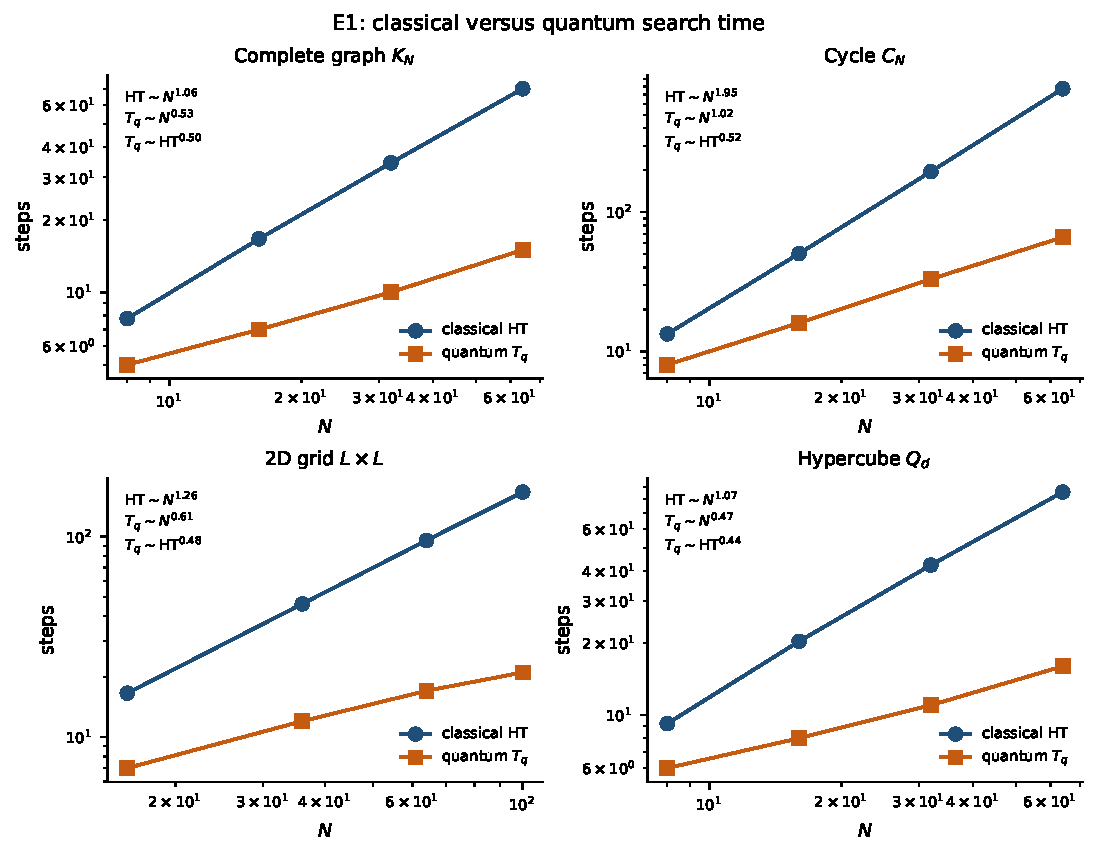
\includegraphics[width=\linewidth]{figures/fig_e1_scaling.pdf}
  \caption{Classical hitting time and quantum search time versus graph size for
  complete graphs, cycles, 2D grids, and hypercubes. Both axes are logarithmic;
  lines are power-law fits. The quantum time tracks a square-root law in the
  classical hitting time rather than in the raw vertex count.}
  \label{fig:e1}
\end{figure}

\begin{table}[t]
  \centering
  \small
  \begin{tabular}{@{}lcccc@{}}
    \toprule
    Family & $\HT\sim N^{\alpha}$ & $T_q\sim N^{\beta}$
    & $T_q\sim \HT^{\gamma}$ & max $\HT/T_q$ \\
    \midrule
    Complete $K_N$ & 1.06 & 0.53 & 0.50 & 4.7 \\
    Cycle $C_N$ & 1.95 & 1.02 & 0.52 & 11.7 \\
    2D grid $L\times L$ & 1.26 & 0.61 & 0.48 & 7.9 \\
    Hypercube $Q_d$ & 1.07 & 0.47 & 0.44 & 5.4 \\
    \bottomrule
  \end{tabular}
  \caption{Fitted scaling exponents from E1. The exponent $\gamma$ is the
  relevant comparison for the AGJK guarantee: it is close to $1/2$ in all four
  families.}
  \label{tab:scaling}
\end{table}

The cycle is the clearest illustration: its classical hitting time grows almost
quadratically ($\alpha=1.95$), while the quantum search time grows almost
linearly ($\beta=1.02$), giving a speedup that reaches $11.7\times$ at $N=64$.
The complete graph ($\HT=\Theta(N)$ exactly) and the hypercube both have
nearly linear hitting times over this size range ($\alpha\approx1.06$--$1.07$),
and the quantum exponents are again close to $1/2$. The grid
shows a slightly larger exponent because the finite-size range does not yet
fully separate $N$ from $\log N$; the fit against $\HT$ gives
$\gamma=0.48$, consistent with the predicted square-root law. The hypercube
has the lowest exponent ($\gamma=0.44$); with only four sizes and integer
$T_q\in\{6,8,11,16\}$ this fit is the least precise of the four.

\FloatBarrier
\subsection{Single, independent, and clustered targets (E2)}
\label{sec:results-e2}

\Cref{fig:e2-success} compares success-probability curves for single,
independent, and clustered marked sets. The independent configuration is
consistently the easiest: on the $8\times8$ grid its mean $\HT$ is $34.7$,
versus $95.5$ for a single target and $79.5$ for a cluster of four. The same
pattern is much stronger on the barbell graph, where independent targets reduce
the hitting time from $2558$ to $16.8$ at $n_{\mathrm{each}}=16$. Clustered
targets give only a modest reduction relative to a single target ($\approx3\%$
on the $n=16$ barbell, $\approx17\%$ on the $8\times8$ grid), far less than
independent targets: once the walker reaches the cluster it still has to find
one of its vertices.

\begin{figure}[t]
  \centering
  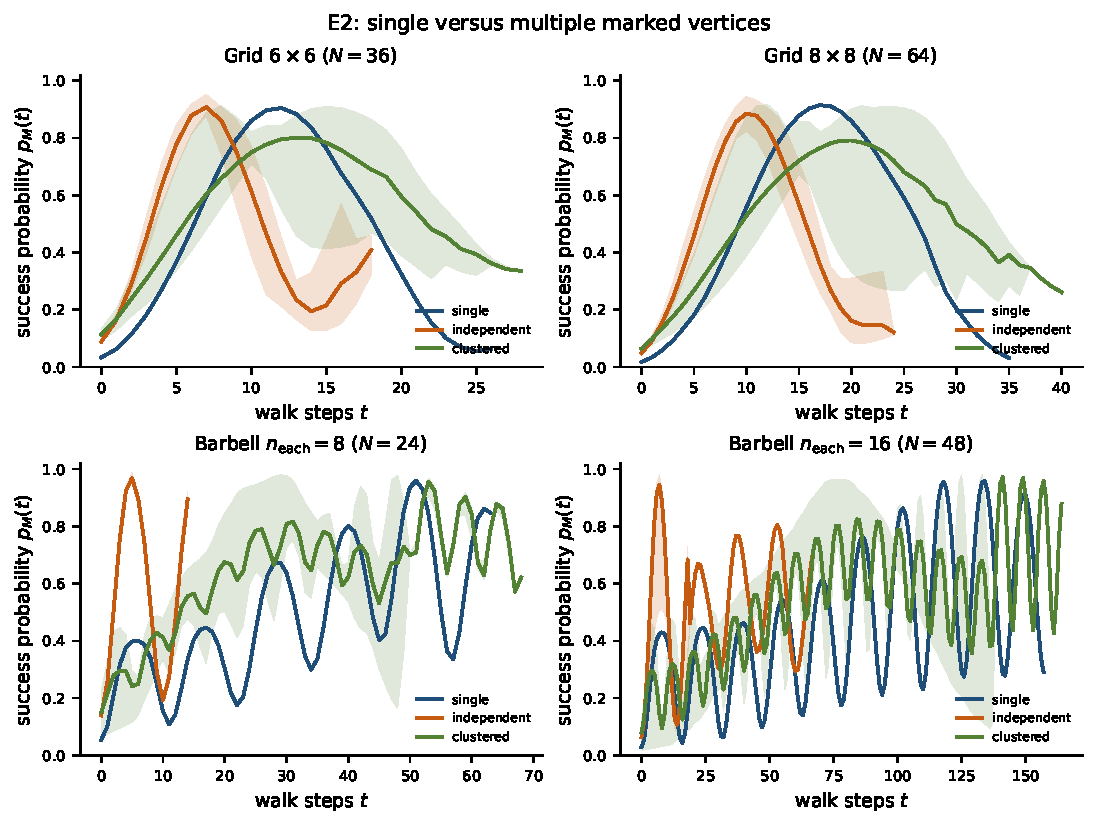
\includegraphics[width=\linewidth]{figures/fig_e2_success.pdf}
  \caption{Success probability versus walk steps for single, independent, and
  clustered marked sets. Shaded bands show the min--max range over three seeds
  (two distinct sets on the $6\times6$ grid and the barbell graphs). Independent targets peak earlier and remain easier; clustered
  targets follow the single-target curve.}
  \label{fig:e2-success}
\end{figure}

\begin{table}[t]
  \centering
  \small
  \begin{tabular}{@{}llcccc@{}}
    \toprule
    Graph & Marked set & mean $\HT$ & mean $\HT^+$ & $\HT^+/\HT$ & mean $T_q$ \\
    \midrule
    Grid $8\times8$ & single & 95.5 & 95.5 & 1.00 & 17.0 \\
    Grid $8\times8$ & independent & 34.7 & 35.3 & 1.02 & 10.7 \\
    Grid $8\times8$ & clustered & 79.5 & 85.3 & 1.07 & 20.3 \\
    Barbell $n=16$ & single & 2558.0 & 2557.9 & 1.00 & 134.0 \\
    Barbell $n=16$ & independent & 16.8 & 25.4 & 1.52 & 7.0 \\
    Barbell $n=16$ & clustered & 2478.6 & 2507.4 & 1.01 & 115.3 \\
    \bottomrule
  \end{tabular}
  \caption{Selected E2 results. Means are over three seeds (0, 1, 2) of farthest-point sampling for the
  independent and clustered configurations; for the $6\times6$ grid and the
  barbell graphs ($n=8,16$) seeds 0 and 2 give the same set, so only two
  distinct sets enter those means.}
  \label{tab:e2}
\end{table}

\Cref{fig:e2-ht} places classical hitting times against extended hitting times.
For the grid and barbell cases the two quantities are close: the largest ratio
is $1.52$ for independent targets on the barbell, where several targets sit in
different communities. The right panel shows the AGJK adversarial torus
construction, where the ratio grows from $5.5$ at $L=18$ to $8.8$ at $L=36$,
consistent with growth but too small a range to establish the asymptotic rate.
This confirms that a large $\HT^+$ penalty is a structural phenomenon: it
requires a particular arrangement of marked vertices, not merely clustering.
For $L=18$ the interpolated walk still reaches $p_{\max}=0.978$ at $t=6$, so the
Conjecture~3 numerical protocol is not slowed down by the large $\HT^+$ value.

\begin{figure}[t]
  \centering
  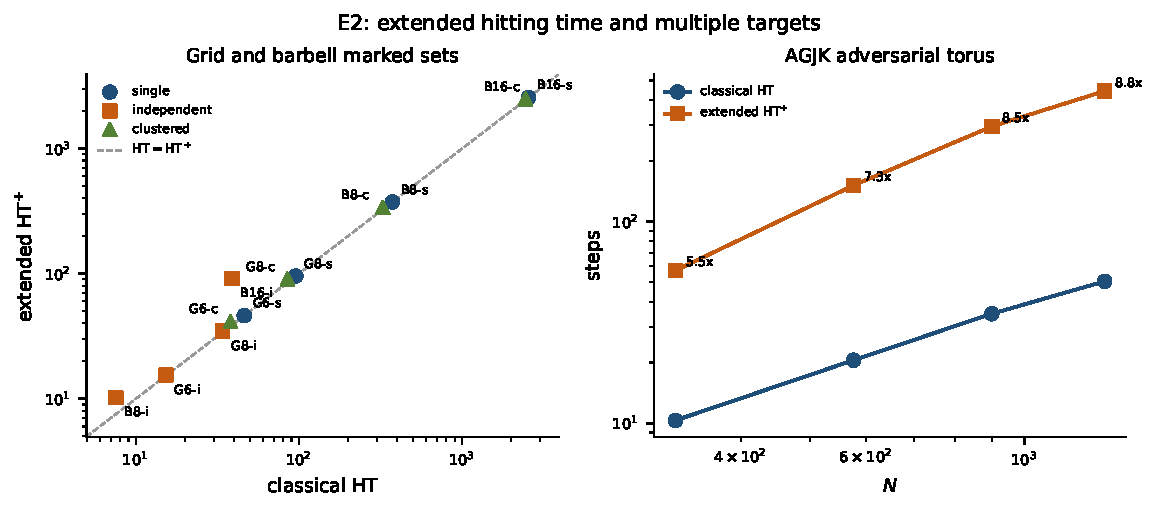
\includegraphics[width=\linewidth]{figures/fig_e2_ht.pdf}
  \caption{Left: classical hitting time versus extended hitting time for the
  grid and barbell marked sets; the dashed line is $\HT=\HT^+$. Right: the AGJK
  adversarial torus construction, where $\HT^+$ grows much faster than $\HT$.
  Labels give the ratio $\HT^+/\HT$.}
  \label{fig:e2-ht}
\end{figure}

\FloatBarrier
\subsection{Semantic activation (E3)}
\label{sec:results-e3}

\Cref{fig:e3} shows the toy semantic graph and the target activation from the
cue \texttt{animal} to two targets: \texttt{dog} (distance $1$) and
\texttt{violin} (distance $4$). The spectral gap is $\lambda_1=0.0333$, giving a
relaxation time of $30.0$ steps. For the near target the CTQW peak is $0.237$ at
$\tau=4.75$, compared with a CRW peak of $0.158$ at $\tau=0.13$. For the far
target the gap is larger: CTQW reaches $0.247$ at $\tau=6.86$, while the CRW
only reaches $0.046$, essentially its stationary value.

\begin{figure}[t]
  \centering
  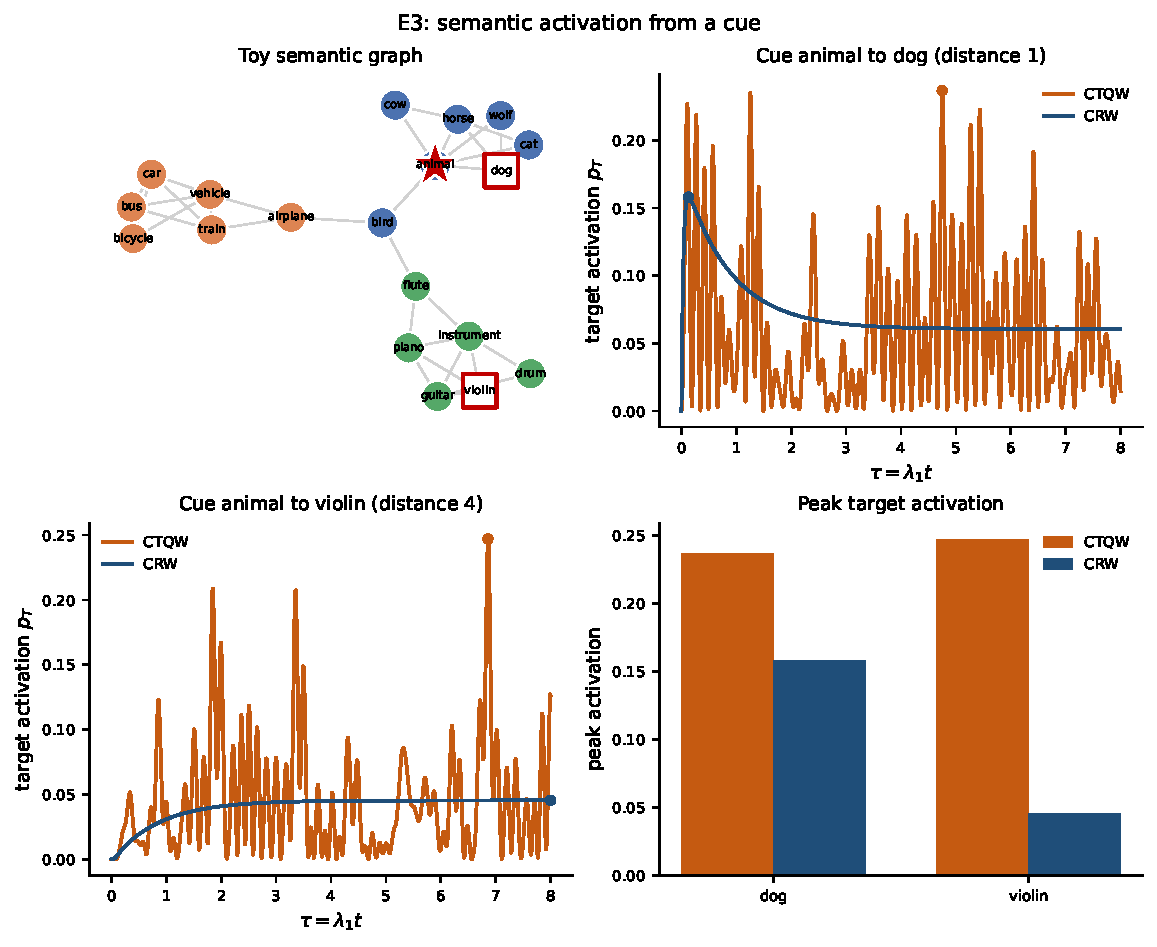
\includegraphics[width=\linewidth]{figures/fig_e3_semantic.pdf}
  \caption{Toy semantic graph and target activation from the cue
  \texttt{animal}. Time is normalized by the spectral gap. The CTQW produces
  larger and later peaks than the CRW, especially for the cross-community
  target \texttt{violin}.}
  \label{fig:e3}
\end{figure}

The activation curves show a clear semantic-distance effect. For the near
target the CRW has a higher area under the curve ($0.580$ versus $0.481$)
because it activates the neighbor immediately and then relaxes. For the far
target the CTQW has a higher AUC ($0.360$ versus $0.324$) and a much higher
peak, while the CRW spreads almost uniformly. The expected radius at the CTQW
peak is also larger ($2.99$ versus $2.36$), indicating that the quantum walk
maintains a broader, more coherent activation pattern instead of collapsing
onto the local neighborhood.

\FloatBarrier
\subsection{Multi-alternative choice under coupling (E4)}
\label{sec:results-e4}

The decision experiment has the same pitfall as E5. Our first readout took
the choice distribution at the first time the total option probability
crossed $0.5$. Because the coherent walk oscillates, that time jumps between
very different phases when the graph changes slightly. Across the laziness
sweep $\eta\in\{0,0.05,0.1,0.2\}$ and ten draws of $\pm20\%$ edge-weight jitter,
the probability of the uncoupled option under this readout moves by a median
of $0.44$ and up to $0.78$ (\cref{fig:e4}, bottom right), so it cannot support
any claim about the effect of coupling. We replace it
with two phase-free quantum readouts: \emph{random stopping}, the choice
distribution averaged over a uniform stopping time $t\in\{1,\dots,400\}$, and
\emph{detection}, in which a position measurement at rate $p=0.2$ per step
ends the decision as soon as it lands on an option terminal.

Under the detection readout the result is stable: the spread is at most
$0.045$, smaller than that of the classical absorbing walk ($0.065$). The
random-stopping readout is in between (median $0.08$, maximum $0.26$).
Both phase-free quantum readouts show the same effect (\cref{fig:e4}): coupling
two options moves probability to the option that is not coupled, and the
shift grows with $c$. Under detection it is monotone in all three graphs;
under random stopping it is monotone up to dips below $0.004$ on the
asymmetric graph. In the symmetric three-option graph the
uncoupled option goes from $1/3$ to $0.499$ at $c=2$ under detection ($0.580$
under random stopping), while the coupled pair falls to $0.250$ each. In the
four-option graph the two uncoupled options together go from $0.500$ to
$0.653$. In the asymmetric ($3$--$4$--$5$) graph the uncoupled short branch
goes from $0.342$ to $0.470$, monotonically.

The classical walk behaves differently. On the symmetric graphs its choice
distribution is exactly uniform for every $c$: coupling only moves probability
between the two coupled branches, which stay symmetric with each other. On the
asymmetric graph coupling mostly redistributes mass inside the coupled pair
(option B rises from $0.32$ to $0.51$, option C falls from $0.26$ to $0.09$) while the uncoupled
option changes little ($0.426$ to $0.409$). The quantum effect is therefore a
qualitative difference, not a matter of degree. Its cost is time: the mean
decision time under detection is $31$--$44$ steps, against $17$--$27$ for the
classical walk, because only one step in five is measured.

\begin{figure}[t]
  \centering
  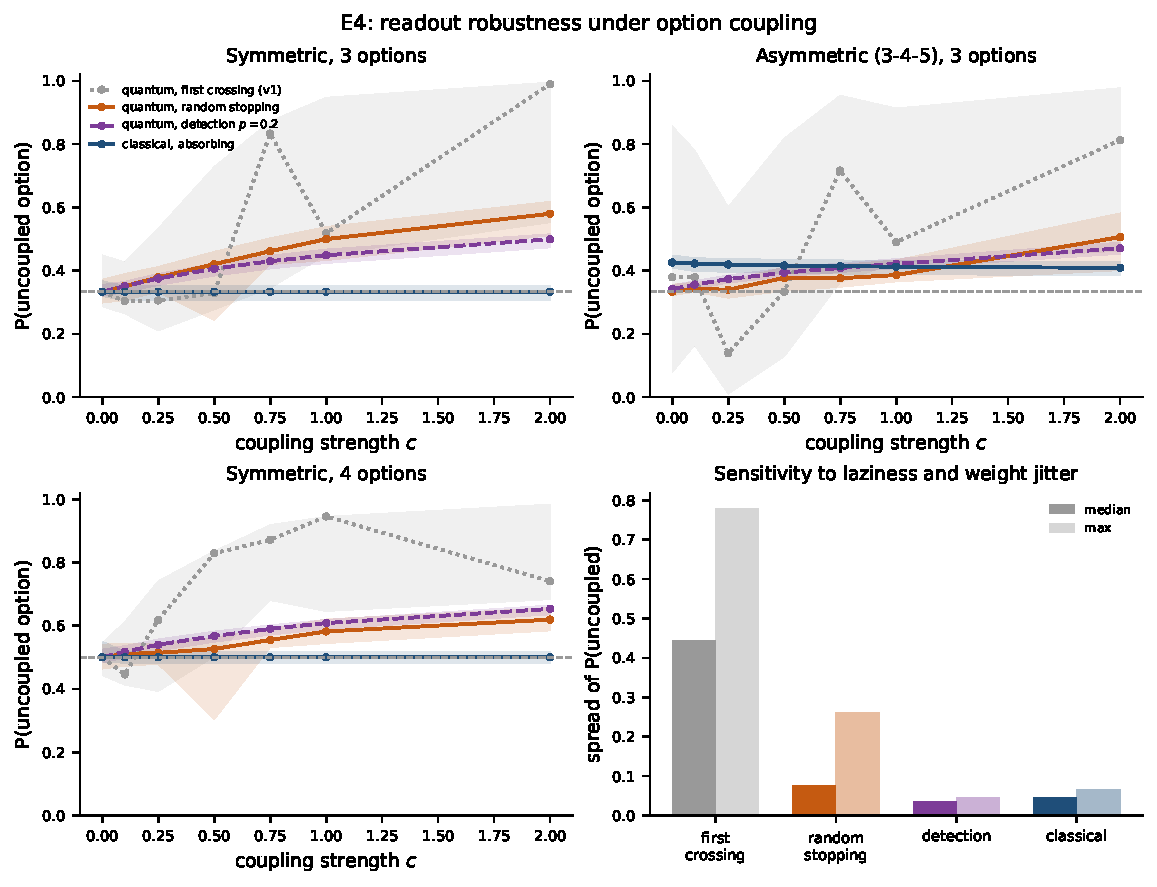
\includegraphics[width=\linewidth]{figures/fig_e4_robustness.pdf}
  \caption{Choice under option coupling. Panels 1--3: probability of the
  uncoupled option(s) versus coupling $c$ for four readouts; lines are the
  nominal graph ($\eta=0.1$), bands span the laziness sweep and edge-weight
  jitter. The dashed grey line is the uniform baseline. Bottom right: spread of
  that probability across variants for each readout.}
  \label{fig:e4}
\end{figure}

This is a model-level analogue of the similarity effect in multi-alternative
choice: when two alternatives become more similar, the dissimilar alternative
gains share. In the walk model it arises from interference between the coupled
branches; the classical walk on the same graph does not produce it.

\FloatBarrier
\subsection{Coherence versus intermediate measurement (E5)}
\label{sec:results-e5}

A pure quantum walk does not approach its target monotonically; its success
probability oscillates. Any comparison at a single deadline therefore depends
on where that deadline falls in the oscillation. The top-left panel of
\cref{fig:e5} makes this explicit for the single-target grid: at $p=0$ the
readout success peaks at $0.449$ at $T=13$ and is only $0.013$ at $T=20$. An
earlier version of this analysis compared measurement rates at $T=20$ only and
reported a $12\times$ gain from measurement; that gain came from the deadline
sitting in a trough. Under the unified lazy walk ($\eta=0.1$), which shifts
the oscillation, the same comparison gives only $1.6\times$, and averaging over
deadlines removes the gain entirely (below). We therefore report two
deadline-free readouts.

\paragraph{Readout model.} Here the observer reads the position once at the
deadline $T$, and intermediate measurements only reset the walk. Averaging the
success over a uniform deadline $T\in\{1,\dots,H\}$ removes the phase
dependence. With $H=120$ the pure walk is best or tied in three of four cases
(grid single $0.042$, grid cluster $0.156$, toy single $0.038$); only the
clustered semantic target gains, from $0.178$ to $0.200$ at $p=0.2$.
Measurement mainly flattens the curve: the coefficient of variation of $p_T$
drops from $1.50$ to $0.37$ on the single-target grid at $p=0.2$. In this
model, measurement buys predictability, not success.

\paragraph{Detection model.} Here a measurement that lands on a marked vertex
ends the search, as in a recognition event, and a final readout is made at the
deadline. Now $p=0$ is the pure walk read once at $T$ and $p=1$ is exactly the
classical first-passage probability $\Pr[\tau_M\le T]$.
\Cref{tab:e5} and the right half of \cref{fig:e5} show the result. Before
$T\approx15$ the pure walk wins in every case, because its first coherent peak
arrives before measurement has had time to help. For clustered targets an
intermediate rate is best for $T\gtrsim20$, apart from single-step revisits of
a later pure-walk peak (e.g.\ $T=35$ on the grid):
$p^\ast=0.2$--$0.3$ finds the cluster by $T=40$ with probability
$0.455$ (grid) and $0.451$ (semantic graph), versus $0.326$ and $0.342$ for the
classical walk and $0.055$ and $0.158$ for the pure walk. By $T=120$ the
advantage over the classical walk is smaller but still present ($0.862$ versus
$0.811$; $0.844$ versus $0.703$). For single targets the optimum moves toward
the classical limit as the deadline grows, though not monotonically: on the
grid $p^\ast$ goes from $0$ (near the first quantum peak) through
$0.2$--$0.5$, with a brief return to $0$ at $T=34$--$36$, to $1$ from $T=71$;
on the semantic graph the classical walk is best for $13\le T\le85$ and within
$0.01$ of the best ($p=0.5$) afterwards.

\begin{figure}[t]
  \centering
  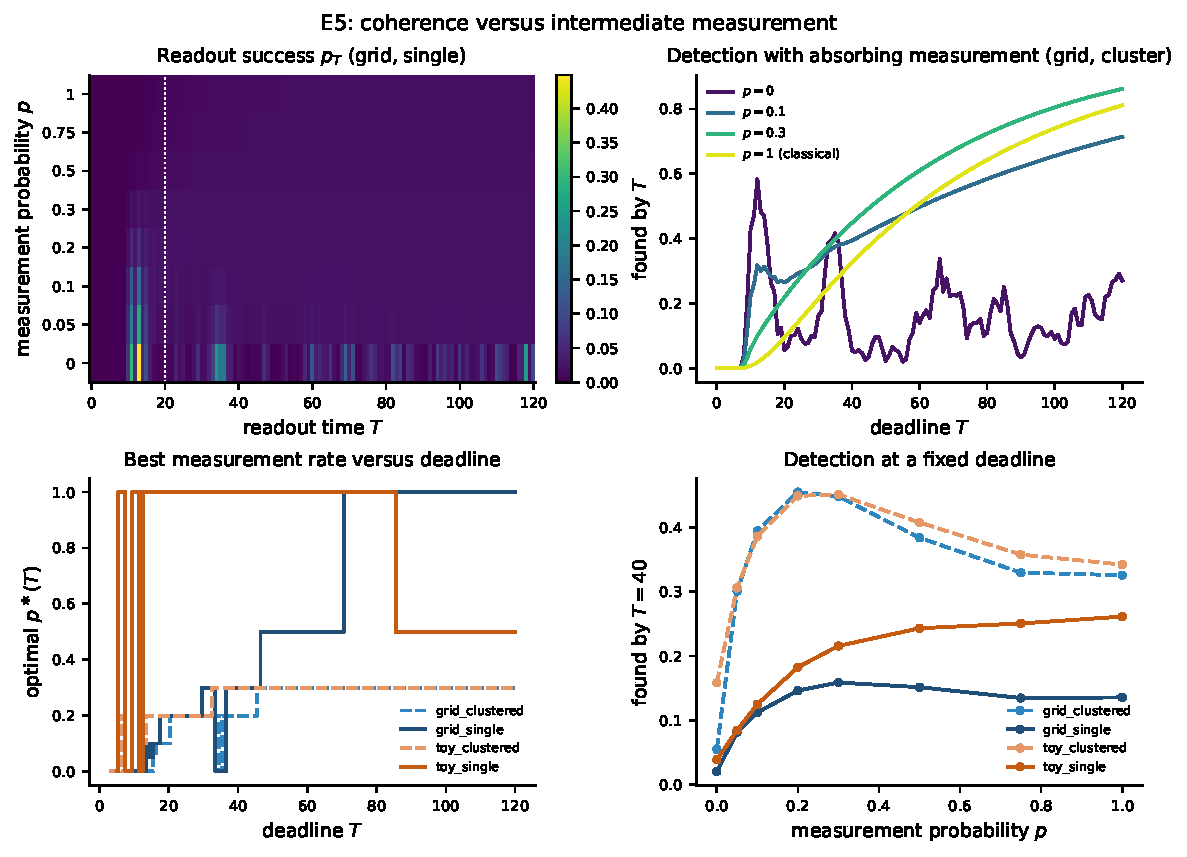
\includegraphics[width=\linewidth]{figures/fig_e5_robustness.pdf}
  \caption{Coherence versus intermediate measurement. Top left: readout
  success $p_T$ on the single-target grid (rows are the tested $p$ values,
  not to scale); the dotted line marks the old deadline $T=20$. Top right: probability that the target cluster has been found
  by $T$ in the detection model. Bottom left: best measurement rate $p^\ast$ as
  a function of the deadline. Bottom right: detection probability at $T=40$
  versus $p$.}
  \label{fig:e5}
\end{figure}

\begin{table}[t]
  \centering
  \small
  \begin{tabular}{@{}lccccc@{}}
    \toprule
    & \multicolumn{2}{c}{pure walk ($p=0$)}
    & \multicolumn{3}{c}{found by $T=40$ (detection model)} \\
    \cmidrule(lr){2-3}\cmidrule(l){4-6}
    Case & peak & at $t$ & $p=0$ & $p=1$ & best $p$ (value) \\
    \midrule
    Grid, single & 0.449 & 13 & 0.020 & 0.136 & 0.3 (0.159) \\
    Grid, clustered & 0.583 & 12 & 0.055 & 0.326 & 0.2 (0.455) \\
    Toy, single & 0.198 & 107 & 0.039 & 0.261 & 1.0 (0.261) \\
    Toy, clustered & 0.394 & 58 & 0.158 & 0.342 & 0.3 (0.451) \\
    \bottomrule
  \end{tabular}
  \caption{E5 summary. The pure walk has the highest peak in every case but
  needs that peak to be timed; with absorbing measurement an intermediate rate
  beats both limits for clustered targets.}
  \label{tab:e5}
\end{table}

The picture is a three-way tradeoff. A perfectly timed coherent search has the
highest peak, the classical walk accumulates detections reliably, and a
partially coherent search combines fast spreading with the ability to stop
once the target is seen. The last option wins when the target is extended
(a cluster of related concepts) and the deadline is moderate.

\FloatBarrier
\subsection{Summary of empirical findings}
\label{sec:results-summary}

The experiments support three conclusions. First, the quantum search time
tracks $\sqrt{\HT}$ across the synthetic families, and independent targets are
easier than clustered ones. Second, a large $\HT^+/\HT$ gap is a structural
effect of the marked-set arrangement, not a generic consequence of having
multiple targets. Third, the cognitive layer is sensitive to graph structure:
semantic distance changes activation timing, option coupling shifts quantum
choice toward the uncoupled option while leaving the classical choice
unchanged, and when a measurement can end the search, an intermediate
measurement rate finds clustered targets faster than either the pure quantum
or the classical walk, even though the pure walk keeps the highest timed peak.

\section{Discussion}
\label{sec:discussion}

\subsection{What the experiments show}
\label{sec:discussion-findings}

The scaling experiments reproduce the central AGJK phenomenon. Across four
graph families the quantum search time fits $T_q\sim\HT^{0.44\text{--}0.52}$,
close to the predicted square-root law, and the peak success probability is
high enough that the fitted times are meaningful. The cycle gives the largest
speedup because its classical hitting time is almost quadratic. The complete
graph and hypercube have smaller finite-size speedups because their classical
hitting times grow almost linearly over the simulated range.

The multiple-target experiments refine the picture. Independent targets are
easier: spreading targets across the graph lowers both the classical hitting
time and the quantum search time. Clustered targets behave like a single
target, because reaching the cluster does not mean finding a particular vertex.
The extended hitting time is close to the classical hitting time for these
configurations. The dramatic $\HT^+\gg\HT$ gap appears only in the periodic
adversarial construction of AGJK. This is an important negative result for a
naive reading of $\HT^+$: multiple targets alone do not create the penalty.
The penalty is a property of the arrangement and of the resulting spectral
structure.

The semantic experiment shows a distance-dependent difference between CTQW and
CRW. For a near target the classical walk activates the neighbor immediately
and has a larger early AUC. For a far target the quantum walk maintains a
larger and later peak, and its activation is spread over a larger radius. This
is consistent with the intuition that coherent propagation can bridge
communities, while classical diffusion relaxes to the stationary distribution.
The result is a model-level prediction: a semantic-search experiment should
see a larger peak but a later response for cross-community targets under the
quantum model, and an earlier but lower activation under the classical model.

The decision experiment produces a context effect that the classical walk
cannot. Coupling two options shifts quantum choice toward the uncoupled
option, increasingly with the coupling strength, while the classical choice on
symmetric graphs stays exactly uniform. The effect is moderate (from $1/3$ to
about $0.5$ on the symmetric three-option graph). Under the detection readout
it is monotone and robust to laziness and edge-weight noise (spread
$\le0.045$); under random stopping it is noisier; under a first-threshold
readout it is swamped by the oscillation phase. This is the same lesson as in
E5: a coherent walk must be read out with a stopping rule that does not depend
on its phase.

The decoherence experiment answers the noise question only once the readout
is specified. Comparing rates at one deadline is unreliable, because the pure
walk oscillates and the comparison then measures the oscillation phase; our
own first analysis made this mistake and reported a $12\times$ gain that
disappears under deadline averaging. If measurement only resets the walk, it
makes the success curve flatter but not higher. If a measurement can also end
the search, the pure walk wins only at short deadlines that catch its first
peak; beyond that an intermediate rate $p\approx0.2$--$0.3$ beats both the pure
quantum and the classical walk for clustered targets, and for single targets
the best rate moves, non-monotonically, toward the classical limit. The
model therefore predicts that the useful amount of ``introspection'' depends
on how extended the target is and how much time is available, which is a
testable prediction for deadline-manipulation experiments.

\subsection{Relation to the literature}
\label{sec:discussion-literature}

The technical results are consistent with AGJK \citep{agjk2019}. Our numerical
protocol tests the simpler interpolated-walk algorithm (Conjecture~3) and cites
the fast-forwarding theorem as the proved guarantee. The adversarial torus
reproduces the qualitative $\HT^+\gg\HT$ behavior and shows that the effect
survives at modest sizes ($L=18$--$36$). We do not claim a new theorem; the
contribution is the numerical validation and the cognitive interpretation.

The semantic experiment is closest to Pavone and Faro \citep{pavone2025}, but
it uses a discrete marked-vertex search perspective rather than an insight
task. The decision experiment is related to Huang and Busemeyer
\citep{huang2022} and to the evidence-accumulation literature
\citep{chen2022}. The decoherence model is a simplified version of the
open-system ideas in Epping et al.\ \citep{epping2023}: projective
measurements at a fixed rate rather than a Lindblad master equation. The
qualitative conclusion---that noise can help at intermediate levels and hurt at
strong levels---is consistent with the broader quantum-cognition literature on
decoherence-assisted processes.

\subsection{Algorithmic versus biological claims}
\label{sec:discussion-claims}

The project is deliberately agnostic about biology. Quantum walks are used as a
mathematical process model, not as a claim that the brain is a quantum computer.
The algorithmic advantage is a statement about the number of walk steps needed
to reach a target under a particular graph and marked set. Whether a biological
system can realize such a walk is a separate question. We keep the two claims
separate throughout: the QIS results concern complexity and spectra, and the
cognitive results concern the qualitative patterns that a process model can
produce.

This separation also limits the interpretation of the context effects. The
decision experiment shows that a quantum walk can produce a similarity-like
shift in choice under option coupling. It does not show that human similarity
effects arise from quantum interference. The value of the model is that it
generates distinct predictions: a classical random walk and a quantum walk on
the same graph produce different choice distributions and different response
times, so an experiment could in principle distinguish them.

\subsection{Limitations}
\label{sec:discussion-limitations}

Several limitations should be stated clearly.
\begin{itemize}[leftmargin=1.4em]
  \item \textbf{No human data.} The experiments are numerical. The cognitive
  quantities are model-defined, not fitted to behavioral data.
  \item \textbf{Synthetic graphs.} The semantic graph is hand-built and small
  ($19$ vertices). It illustrates the mechanism but does not capture the scale
  or noise of real semantic memory.
  \item \textbf{Interpolation selection.} The parameter $s$ is chosen by a
  grid search on the AGJK lower bound. A different selection rule could change
  the constants in the search times, although the scaling exponents are stable.
  \item \textbf{Two walk formalisms.} The search experiments use discrete-time
  Szegedy walks, while the semantic experiment uses continuous-time walks. We
  compare them only within their own time normalizations and do not mix the
  two formalisms in a single fit.
  \item \textbf{Simplified noise.} The decoherence model uses projective
  position measurements and resets. It is not a full Lindblad or open-system
  model.
  \item \textbf{Finite sizes.} The graphs have at most a few hundred vertices.
  The asymptotic exponents are estimated from small ranges, especially for the
  grid and hypercube.
\end{itemize}

\subsection{Future work}
\label{sec:discussion-future}

Four extensions would strengthen the project. First, replace the toy semantic
graph with a ConceptNet subgraph and test whether the distance-dependent
activation pattern survives in a real semantic network. Second, fit the
decision model to behavioral choice and response-time data, using the coupling
parameter as a free similarity parameter. Third, replace the projective
measurement model with a Lindblad equation or a continuous dephasing model and
compare the optimal noise level. Fourth, implement the decision graph on a
small quantum device or circuit simulator to test whether the context effect
survives realistic noise. A larger graph study could also test how the size
of the context effect depends on branch lengths, coupling patterns, and the
measurement rate of the detection readout.

\section{Conclusion}
\label{sec:conclusion}

This project used the AGJK marked-vertex search algorithm as the QIS core of a
process-level model of cognitive search. We implemented the Szegedy and
interpolated walks, verified the $\widetilde O(\sqrt{\HT})$ scaling on four
graph families, and compared single, independent, and clustered targets. The
main structural finding is that independent targets are easier, while clustered
targets give only a modest reduction relative to a single target ($\approx3\%$
on the barbell, $\approx17\%$ on the $8\times8$ grid); the large $\HT^+\gg\HT$ gap requires the
adversarial periodic arrangement of AGJK rather than clustering alone. On the
cognitive side, a toy semantic graph produced distance-dependent activation
patterns, a multi-branch decision graph produced a robust similarity-like
context effect under option coupling that the classical walk lacks, and a partial-measurement model showed
that, beyond the shortest deadlines, an intermediate measurement rate that can
stop the search finds clustered targets faster than both the pure quantum and
the classical walk.

The broader lesson is that the algorithmic structure of quantum walk search is
a useful source of cognitive hypotheses. The marked-set structure, the
extended hitting time, and the success curve are not merely complexity
quantities; they define a process model with testable predictions. At the same
time, the project is deliberately cautious: the results are numerical,
model-level, and do not claim a biological quantum advantage. The next step is
to test the same predictions on larger semantic networks and, eventually, on
behavioral choice and response-time data.


\section*{AI Tool Usage}
An AI coding assistant was used for code scaffolding, experiment automation,
and LaTeX drafting. All technical derivations, experiment design, numerical
results, and interpretations were checked by the authors. The AI tool was not
used to generate research results or citations without verification.

\appendix
\section{Hitting-time derivations}
\label{app:hitting}

\paragraph{Complete graph.}
For $K_N$ with one marked vertex, every unmarked vertex is equivalent. Let $h$
be the expected hitting time from an unmarked vertex. Then
\begin{equation}
  h=1+\frac{N-2}{N-1}h,
\end{equation}
so $h=N-1$. Since the stationary distribution is uniform and we condition on
starting outside the marked set, $\HT=N-1$.

\paragraph{Cycle.}
For $C_N$ with marked vertex $0$, the expected hitting time from distance $i$ is
$h_i=i(N-i)$. It satisfies the recurrence
\begin{equation}
  h_i=1+\frac{1}{2}h_{i-1}+\frac{1}{2}h_{i+1},\qquad h_0=h_N=0,
\end{equation}
whose solution is the quadratic above. Averaging over
$i=1,\dots,N-1$ gives
\begin{equation}
  \HT=\frac{1}{N-1}\sum_{i=1}^{N-1}i(N-i)=\frac{N(N+1)}{6}.
\end{equation}
These identities are used as sanity checks in \texttt{tests/test\_classical.py}.

\section{Discriminant matrix and spectral identity}
\label{app:discriminant}

For a reversible chain, detailed balance gives
$\pi_xP_{xy}=\pi_yP_{yx}$, hence
\begin{equation}
  D_{xy}=\sqrt{P_{xy}P_{yx}}
  =\frac{\sqrt{\pi_x}P_{xy}}{\sqrt{\pi_y}},
\end{equation}
so $D=\mathrm{diag}(\pi)^{1/2}P\,\mathrm{diag}(\pi)^{-1/2}$. The matrices $D$
and $P$ are similar, so they have the same eigenvalues, and $D$ is symmetric.
The identity
\begin{equation}
  \langle\bar0|\langle x|W(P)|\bar0\rangle|y\rangle
  =\sqrt{P_{xy}P_{yx}}=D_{xy}
\end{equation}
follows directly from the definitions of $V(P)$, $\mathrm{Shift}$, and
$\mathrm{Ref}$. For the interpolated walk, the same computation gives the
top-left block $D(s)$, which is the starting point for the Chebyshev bound
\eqref{eq:chebyshev}.

\section{Measurement ensemble recursion}
\label{app:measurement}

Let $\lvert\phi_{x,a}\rangle=W(0)^a\lvert\bar0\rangle\lvert x\rangle$ for
$a=0,\dots,T_{\max}$, with position marginal
$\mu_{x,a}(y)=\lVert\Pi_y\lvert\phi_{x,a}\rangle\rVert^2$ and marked mass
$s_{x,a}=\sum_{y\in M}\mu_{x,a}(y)$. Let $\mu^{(0)}_a$ and $s^{(0)}_a$ be the
corresponding quantities for the initial state. A trajectory is described by
$q_0(t)$, the probability that no measurement has occurred by time $t$, and by
$q_{x,a}(t)$, the probability that the last reset was at vertex $x$ and the
state has evolved for $a$ steps since that reset.

At one step,
\begin{align}
  q_0(t+1)&=(1-p)q_0(t),\\
  q_{x,a+1}(t+1)&=(1-p)q_{x,a}(t),\\
  q_{y,1}(t+1)&=p\,q_0(t)\mu^{(0)}_t(y)
  +p\sum_{x,a}q_{x,a}(t)\mu_{x,a}(y).
\end{align}
The success probability is
\begin{equation}
  p_M(t+1)=q_0(t+1)s^{(0)}_{t+1}
  +\sum_{x,a}q_{x,a}(t+1)s_{x,a}.
\end{equation}
This recursion is exact for the channel \eqref{eq:measurement-channel}. It
requires the basis ensembles once per graph and marked set, after which a
sweep over $p$ is inexpensive. The implementation is in
\texttt{src/noise.py}.

For the detection model, the mass that a measurement places on $M$ is removed
instead of reset. With $f(t)$ the probability found by time $t$,
\begin{align}
  f(t+1)&=f(t)+p\sum_{y\in M}\Bigl[q_0(t)\mu^{(0)}_t(y)
  +\sum_{x,a}q_{x,a}(t)\mu_{x,a}(y)\Bigr],
\end{align}
the reset term $q_{y,1}(t+1)$ is restricted to $y\notin M$, and the probability
of having found the target with a final readout at $T$ is
$F_p(T)=f(T)+q_0(T)s^{(0)}_T+\sum_{x,a}q_{x,a}(T)s_{x,a}$.

\section{Additional results}
\label{app:additional}

\Cref{fig:e1-speedup} shows the classical-to-quantum speedup for E1. The cycle
has the largest speedup because its classical hitting time grows almost
quadratically; the complete graph has the smallest because its classical
hitting time grows only linearly.

\begin{figure}[t]
  \centering
  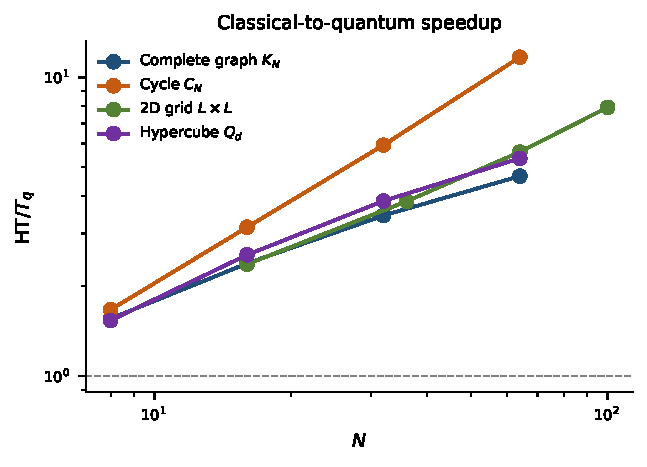
\includegraphics[width=0.72\linewidth]{figures/fig_e1_speedup.pdf}
  \caption{Classical-to-quantum speedup $\HT/T_q$ versus graph size for E1.}
  \label{fig:e1-speedup}
\end{figure}

\begin{table}[t]
  \centering
  \small
  \begin{tabular}{@{}llccccc@{}}
    \toprule
    Graph & Marked set & sets & median $\HT$ [min, max] & median $\HT^+/\HT$ & max $\HT^+/\HT$ & median $T_q$ \\
    \midrule
    Grid $6\times6$ & single & 1 & 46.1 & 1.00 & 1.00 & 12 \\
    Grid $6\times6$ & independent & 14 & 15.7 [12.7, 17.4] & 1.01 & 1.02 & 7 \\
    Grid $6\times6$ & clustered & 17 & 40.1 [17.6, 54.9] & 1.09 & 1.10 & 14 \\
    Grid $8\times8$ & single & 1 & 95.5 & 1.00 & 1.00 & 17 \\
    Grid $8\times8$ & independent & 18 & 34.8 [26.9, 39.7] & 1.02 & 1.05 & 10 \\
    Grid $8\times8$ & clustered & 18 & 85.0 [41.5, 131.1] & 1.06 & 1.09 & 20 \\
    Barbell $n=8$ & single & 1 & 373.6 & 1.00 & 1.00 & 51 \\
    Barbell $n=8$ & independent & 11 & 7.6 [7.1, 7.6] & 1.38 & 1.38 & 5 \\
    Barbell $n=8$ & clustered & 9 & 425.3 [196.6, 433.2] & 1.01 & 1.09 & 48 \\
    Barbell $n=16$ & single & 1 & 2558.0 & 1.00 & 1.00 & 134 \\
    Barbell $n=16$ & independent & 18 & 16.8 [16.4, 415.1] & 1.53 & 2.94 & 7 \\
    Barbell $n=16$ & clustered & 16 & 2768.0 [1893.1, 2781.3] & 1.00 & 1.04 & 133 \\
    \bottomrule
  \end{tabular}
  \caption{Full E2 results. Single targets have one set; other rows summarize
  all distinct sets from seeds $0,\dots,19$.}
  \label{tab:e2-full}
\end{table}

\section{Reproducibility}
\label{app:reproducibility}

The environment is created with
\begin{verbatim}
mamba env create -f environment.yml
mamba activate qwalk-cognition
\end{verbatim}
from \texttt{Final/code}. Everything is reproduced from \texttt{Final/code} with
\begin{verbatim}
make all
\end{verbatim}
which runs the tests, all six experiments, copies the figures used in the paper,
writes \texttt{results/MANIFEST.json} (git commit, dirty-tree flag, package
versions, and SHA-256 checksums of configs and results), and compiles the report.
Single experiments can be run with, for example,
\texttt{python -m src.experiments --only E6}. The complete run takes about
fifteen minutes, most of it in E4's robustness sweep. The test suite contains 71
passing tests. The configuration files are \texttt{configs/base.yaml} and
\texttt{configs/experiments.yaml}; all random choices use explicit seeds.


\bibliographystyle{plainnat}
\bibliography{refs}

\end{document}
